\documentclass[a4paper,12pt]{article}
\usepackage[utf8]{inputenc}
\usepackage[spanish]{babel}
\usepackage{color}
\usepackage{parskip}
\usepackage{graphicx}
\usepackage{multirow}
\usepackage{listings}
\usepackage{vmargin}
\usepackage{datetime}
\newdate{date}{07}{12}{2017}
\graphicspath{ {imagenes/} }
\definecolor{mygreen}{rgb}{0,0.6,0}
\definecolor{lbcolor}{rgb}{0.9,0.9,0.9}
\usepackage{epstopdf}
\usepackage{float}


\setpapersize{A4}
\setmargins{2.5cm}       % margen izquierdo
{1.5cm}                        % margen superior
{16.5cm}                      % anchura del texto
{23.42cm}                    % altura del texto
{10pt}                           % altura de los encabezados
{1cm}                           % espacio entre el texto y los encabezados
{0pt}                             % altura del pie de página
{2cm}     

\lstset{
    tabsize=4,    
%   rulecolor=,
    language=[GNU]C++,
        basicstyle=\tiny,
        aboveskip={1.5\baselineskip},
        columns=fixed,
        showstringspaces=false,
        extendedchars=false,
        breaklines=true,
        prebreak = \raisebox{0ex}[0ex][0ex]{\ensuremath{\hookleftarrow}},
        frame=single,
        showtabs=false,
        showspaces=false,
        showstringspaces=false,
        identifierstyle=\ttfamily,
        keywordstyle=\color[rgb]{0,0,1},
        commentstyle=\color[rgb]{0.026,0.112,0.095},
        stringstyle=\color{red},
        numberstyle=\color[rgb]{0.205, 0.142, 0.73},
%        \lstdefinestyle{C++}{language=C++,style=numbers}’.
}


\begin{document}
\title{Ejercicio del Examen}
\author{
Christofer Fabián Chávez Carazas \\
\small{Universidad Nacional de San Agustín de Arequipa} \\
\small{Escuela Profesional de Ciencia de la Computación} \\
\small{Computación Gráfica}
}
\date{\displaydate{date}}

\maketitle

\begin{large}
 \textbf{Problema}
\end{large}

Realizar un programa el cual reciba un patrón y rellene un polígono con dicho patrón.

\begin{large}
 \textbf{Resultado}
\end{large}

El algoritmo usa la estructura \textit{Matrix} que contiene el borde de un polígono. Esta estructura ya ha sido utilizada en anteriores laboratorios.
La estructura \textit{Patron} en una vector de vectores de boleanos, si es 0 no se pinta, si es 1 sí se pinta.

\begin{itemize}
 \item \textbf{Algoritmo}
 \begin{lstlisting}
void fillFigureWithPatron(Matrix matrix, Patron patron, int color){
    changeColor(color);
    Point actual;
    actual.x = matrix.xMin + 1;
    actual.y = matrix.yMax - 1;
    int actualFil = 0;
    int actualCol = 0;
    while(actual.y > matrix.yMin){
        while(actual.x < matrix.xMax){
            if(matrix.matrix[abs(actual.y - matrix.size.height - 1)][actual.x] == 1) break;
            else if(patron[actualFil][actualCol] == true) drawPoint(actual);  
            actual.x++;
            actualCol++;
            if(actualCol == patron[0].size()) actualCol = 0;
        }
        actual.x = matrix.xMin + 1;
        actual.y--;
        actualFil++;
        if(actualFil == patron.size()) actualFil = 0;
    }
}
 \end{lstlisting}
 \item \textbf{main.cpp}
 \begin{lstlisting}
#include <GL/glut.h>
#include <iostream>
#include <tuple>
#include <cstdlib>
#include <ctime>
#include "primitivas.h"

using namespace std;

GLsizei winWidth = 1200, winHeight = 800;
Window window;

Patron patron = {{0,0,0,0,0,0,0,0,0},
                 {0,1,0,0,0,0,0,1,0},
                 {0,1,1,0,0,0,1,1,0},
                 {0,1,0,1,0,1,0,1,0},
                 {0,1,0,0,1,0,0,1,0},
                 {0,1,0,1,0,1,0,1,0},
                 {0,1,1,0,0,0,1,1,0},
                 {0,1,0,0,0,0,0,1,0},
                 {0,0,0,0,0,0,0,0,0}};


void init(void){
    glClearColor(1.0,1.0,1.0,1.0);
    glMatrixMode(GL_PROJECTION);
    gluOrtho2D(0.0, 1200.0, 0.0, 800.0);
}

void display(void){
    glClear(GL_COLOR_BUFFER_BIT);	
    changeColor(ROJO);
    Point iniRec;
    iniRec.x = 150; iniRec.y = 150;
    Point finRec;
    finRec.x = 300; finRec.y = 300;
    Matrix rectangle = drawRectangle(iniRec, finRec, window);
    fillFigureWithPatron(rectangle, patron, AZUL);
    glFlush();
}


int main(int argc, char **argv){
    srand (time(NULL));
    glutInit(&argc, argv);
    glutInitDisplayMode(GLUT_SINGLE | GLUT_RGB);
    glutInitWindowSize(winWidth, winHeight);
    window.height = winHeight;
    window.width = winWidth;
    glutInitWindowPosition(100, 100);
    glutCreateWindow("Programa Primitivas");
    init();
    glutDisplayFunc(display);


    glutMainLoop();
    return 0;
}
 \end{lstlisting}
\end{itemize}

\begin{figure}[H]
 \centering
 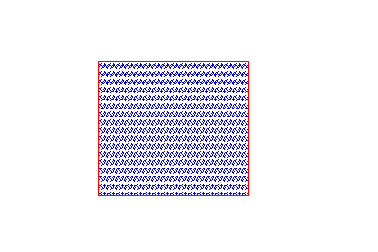
\includegraphics[scale = 0.5]{1.png}
 \caption{Resultados del algoritmo}
\end{figure}





\end{document}

